\documentclass[twoside]{article}
\input{ISC18-english.sty}
\usepackage{float}
\setlength{\textfloatsep}{8pt plus 2pt minus 2pt}
\setlength{\floatsep}{6pt plus 2pt minus 2pt}
\setlength{\intextsep}{8pt plus 2pt minus 2pt}
\setlength{\abovecaptionskip}{4pt}
\setlength{\belowcaptionskip}{0pt}
\begin{document}
\thispagestyle{empty}

%%%%%%%%%%%%%%%%% Article title header  %%%%%%%%%%%%%%%%%%%%
\fancyhead[LE]{Comparison of RK and Smoothing Splines for Soil Zn}
%%%%%%%%%%%%%%%%% Article authors header   %%%%%%%%%%%%%%%%%%%%
\fancyhead[RO]{Alimohammadi,Mahdioun}

\begin{center}
{
\includegraphics [height=25mm, width=150.3mm] {Images/isc18E}} \\
\vspace*{-1.8cm}
\vspace*{4cm}

%%%%%%%%%%%%%%%%% Article title  %%%%%%%%%%%%%%%%%%%%
{\Large \bf Comparative Evaluation of Regression Kriging and Smoothing Splines for Spatial Prediction of Soil Zinc Contamination}\\

\vspace{0.5cm}

%%%%%%%%%%%%%%%%% Article authors and affiliations %%%%%%%%%%%%%%%%%%%%
{\bf
Roshanak Alimohammadi $^1$, Fatemeh Mahdioun \footnote[2]{{\bf Corresponding Author:} {\tt F.Mahdioun@alzahra.ac.ir }} \\
$^1$Department of statistics, Faculty of Mathematical Sciences, Alzahra University \\
$^2$Department of statistics, Faculty of Mathematical Sciences, Alzahra University}
\end{center}

\rule{\textwidth}{0.2mm}\\

%%%%%%%%%%%%%%%%% Article abstract  %%%%%%%%%%%%%%%%%%%%
\noindent{\bf Abstract}\\
Accurate mapping of soil contamination is essential for environmental assessment and remediation planning. This study compares Regression Kriging (RK) and Smoothing Splines (SS) for estimating zinc (Zn) concentrations in the Meuse River Basin using distance from river as an environmental covariate. Variogram analysis indicated a strong spatial structure, with a nugget effect of 0.0356, a total sill of 0.2866, and a range of 267.3\,m. Model performance was evaluated through leave-one-out cross-validation (LOOCV). The results showed that RK outperformed SS, yielding lower RMSE (RK:0.3868 vs.\ SS:0.3989) and MAE (RK:0.2811 vs.\ SS:0.2966). By integrating regression with geostatistical modeling of residuals, RK provided more accurate predictions and better identified local contamination hotspots. These findings highlight the advantage of hybrid geostatistical approaches for spatial modeling of heavy-metal pollution in river-basin environments.

\vspace{0.3cm}
\noindent{\bf Keywords:}
Regression Kriging, Smoothing Spline, Spatial Autocorrelation, Auxiliary Variable, Digital Soil Mapping, Soil Contamination. \\

\noindent{\bf Mathematics Subject Classification (2010):} $\rm 62H11$. \\
\hspace{1cm}\rule{\textwidth}{0.2mm}
%%%%%%%%%%%%%%%%%%%%%%%% Introduction %%%%%%%%%%%%%%%%%%%%%%%%%%%%%
\section{Introduction}
Effective land management and environmental monitoring-especially regarding soil heavy metal contamination-rely heavily on accurate, spatially continuous zoning maps. However, due to budget constraints and logistical hurdles, field sampling is typically restricted to discrete, sparsely distributed locations. To bridge these gaps, spatial interpolation has become an essential tool in environmental science, allowing researchers to transform isolated point observations into comprehensive surfaces. The core challenge, however, remains the same: selecting an interpolation model that can reconstruct complex spatial variability while keeping prediction errors to an absolute minimum. Over the past few decades, the field has largely divided into two camps: geostatistical methods, which leverage spatial autocorrelation, and deterministic or spline-based approaches, which prioritize mathematical smoothness and continuity. Among the more advanced hybrid techniques is RK---also known as universal kriging or kriging with external drift. The logic behind RK is that the spatial variability of an environmental variable, such as soil zinc levels, can be decomposed into two parts: a deterministic trend driven by auxiliary factors (like elevation or distance from a river) and a stochastic residual that still carries a spatial structure. In practice, RK first uses regression to model the relationship between the target variable and its environmental predictors. The remaining residuals, which still exhibit spatial dependence, are then interpolated via simple kriging and merged back into the regression results. By integrating this ancillary environmental data, RK aims to sharpen predictions at unsampled sites and minimize the biases often found in traditional kriging \cite{Hengl2007}. On the other end of the spectrum is SS, a deterministic, non-parametric approach. Unlike probabilistic geostatistics, splines use piecewise functions to create a smooth surface that approximates the data. While classical splines are forced to pass exactly through every sample point, smoothing splines introduce a penalty parameter ($\lambda$) to strike a balance between fitting the observed data and maintaining a smooth overall surface. This is achieved by minimizing a functional that penalizes excessive curvature. SS is particularly useful when dealing with noisy data or when the goal is to capture broad spatial trends without the mathematical heavy lifting of variogram modeling. Because it doesn't require strict assumptions like second-order stationarity, it has become a go-to for rapid spatial modeling\cite{Wahba1990}. Despite the popularity of both methods, a key question persists: when environmental variables are strongly correlated with the pollutant, does the added complexity of RK actually produce better results than the elegant simplicity of Spline Smoothing? Most existing literature compares ordinary kriging to splines, but few studies have directly pitted RK---which utilizes auxiliary predictors---against two-dimensional ss. The Meuse River Basin, with its sharp spatial gradients and well-documented environmental drivers, offers the perfect laboratory to test this. This research evaluates both approaches using quantitative metrics like RMSE and MAE, alongside a visual critique of the resulting maps, to determine the most reliable method for digital environmental mapping in this region.
%%%%%%%%%%%%%%%%%%%%%%%% Materials and Methods %%%%%%%%%%%%%%%%%%%%%%%%%%%%%
\section{Methods}
\subsection{Data}
This research utilizes the well-established Meuse River dataset from the southern Netherlands. The data includes zinc (Zn) concentration measurements from 155 topsoil sampling locations. Because heavy metal concentrations in soil typically exhibit a positive skew, we applied a natural logarithmic ($\ln$) transformation to the raw data. This step was essential to stabilize variance and ensure the residuals aligned more closely with the normality assumptions required for robust regression and geostatistical modeling.

To account for large-scale spatial trends, we used ``distance to the river'' as a primary auxiliary predictor. In the Meuse floodplain, proximity to the river is a dominant factor influencing the deposition and accumulation patterns of pollutants, making it a highly relevant covariate for this study.
\subsection{RK}
RK is a hybrid geostatistical technique that treats spatial variation as a combination of two distinct parts: a deterministic trend and a stochastic residual. The final prediction at any unsampled location ($s_0$) is calculated as the sum of these two components:
\begin{equation}
\hat{Z}(s_0) = \hat{m}(s_0) + \hat{e}(s_0)
\end{equation}
Where $\hat{m}(s_0)$ is the deterministic trend---estimated here through a regression model using the river distance---and $\hat{e}(s_0)$ represents the spatially autocorrelated residuals. 

Our implementation followed a two-step sequence. First, the regression coefficients ($\beta$) were calculated using Ordinary Least Squares (OLS) to establish the global trend. The resulting residuals ($e = Z - \hat{m}$) were then extracted for variogram analysis. We selected an exponential variogram model to characterize the spatial dependence of these residuals, which were subsequently interpolated using Simple Kriging and added back to the regression-based trend.
\subsection{SS}
As a non-parametric alternative, we employed SS, typically formulated within a Generalized Additive Model (GAM) framework. The goal of this method is to fit a smooth surface, $f(x,y)$, that captures the underlying spatial structure of the data by minimizing the following objective function:
\begin{equation}
\sum_{i=1}^n \{z_i - f(x_i, y_i)\}^2 + \lambda J(f)
\end{equation}
In this equation, the first term represents the residual sum of squares (RSS), while $J(f)$ is a roughness penalty that discourages excessive curvature or unrealistic oscillations in the fitted surface. The smoothing parameter, $\lambda$, is critical as it dictates the balance between fitting the observed data and maintaining surface smoothness. To avoid the risks of over-fitting or over-smoothing, we determined the optimal $\lambda$ automatically using the Generalized Cross-Validation (GCV) criterion.
\subsection{Validation}
To rigorously compare the predictive performance of RK and SS, we used a Leave-One-Out Cross-Validation (LOOCV) strategy. Two standard statistical metrics were used for quantification:

\begin{enumerate}
    \item \textbf{Root Mean Square Error (RMSE):} A measure of overall accuracy sensitive to large errors:
    \begin{equation}
    RMSE = \sqrt{\frac{1}{n} \sum_{i=1}^{n} (Z_i - \hat{Z}_i)^2}
    \end{equation}
    \item \textbf{Mean Absolute Error (MAE):} The average magnitude of the errors:
    \begin{equation}
    MAE = \frac{1}{n} \sum_{i=1}^{n} |Z_i - \hat{Z}_i|
    \end{equation}
\end{enumerate}
Lower values in both metrics indicate superior predictive performance. All statistical computations and map visualizations were performed in \texttt{R}, leveraging the \texttt{gstat}, \texttt{mgcv}, and \texttt{sp} packages.
%%%%%%%%%%%%%%%%%%%%%%%% Results and Discussion %%%%%%%%%%%%%%%%%%%%%%%%%%%%%
\section{Analysis of Data Using the Proposed Method}
Zinc (Zn) concentrations in the study area exhibited a marked positive skewness, which is typical for environmental heavy-metal datasets. To stabilize the variance and improve conformity with distributional assumptions commonly required in regression-based modeling, a natural logarithmic transformation ($\ln$) was applied to Zn values prior to analysis. This transformation reduced the influence of extreme observations and provided a more suitable basis for both RK and SS modeling on a comparable scale.

Following the trend modeling stage in RK, the residual component was assessed to determine whether a spatially structured signal remained. The empirical variogram of the regression residuals indicated pronounced spatial autocorrelation, confirming that the residuals were not purely random noise. An exponential variogram model was fitted and subsequently used as the core spatial structure for interpolating residuals within the RK framework. The estimated parameters of the fitted model are reported in Table~\ref{tab:variogram_params}. The nugget-to-sill ratio equals 12.4\%, implying strong spatial dependence and indicating that most of the residual variability is spatially structured rather than measurement error or microscale randomness. The effective correlation range was estimated at 267.3~m, suggesting that samples separated by distances shorter than this threshold tend to be more similar, while dependence diminishes beyond it. These results provide direct methodological support for adopting a geostatistical correction to the regression trend.

\begin{table}[h]
\centering
\caption{Estimated parameters of the exponential variogram model fitted to RK residuals.}
\label{tab:variogram_params}
\begin{tabular}{lc}
\hline
\textbf{Parameter} & \textbf{Value} \\
\hline
Nugget effect & 0.0356 \\
Partial sill & 0.2510 \\
Total sill & 0.2866 \\
Range (m) & 267.2980 \\
Nugget-to-sill ratio (\%) & 12.4 \\
\hline
\end{tabular}
\end{table}

To compare predictive performance, both RK and SS were evaluated using a Leave-One-Out Cross-Validation (LOOCV) procedure. This strategy iteratively removes each observation, predicts it from the remaining data, and summarizes prediction errors across all hold-out cases, thereby providing a robust and nearly unbiased estimate of generalization accuracy. Table~\ref{tab:comparison} reports RMSE and MAE for both methods. RK achieved lower RMSE (0.3868) and lower MAE (0.2811) than SS (RMSE = 0.3989; MAE = 0.2966), indicating a consistent improvement in predictive accuracy. Although the numerical differences are moderate, the superiority of RK across both metrics suggests that explicitly combining a deterministic component with a spatially correlated residual correction yields more reliable estimates than a purely smoothing-based surface.

\begin{table}[h]
\centering
\caption{Comparison of error statistics for the two studied models (LOOCV).}
\label{tab:comparison}
\begin{tabular}{lcc}
\hline
\textbf{Evaluation Metric} & \textbf{Regression Kriging (RK)} & \textbf{Smoothing Splines (SS)} \\
\hline
Root Mean Square Error (RMSE) & 0.3868 & 0.3989 \\
Mean Absolute Error (MAE) & 0.2811 & 0.2966 \\
\hline
\end{tabular}
\end{table}

The spatial prediction maps are presented in Figure~\ref{fig1}. The RK map preserves stronger local contrasts and delineates irregular zone boundaries more distinctly, which is consistent with the model design that combines a covariate-driven trend with residual kriging. In comparison, the SS map displays a smoother and more generalized surface, emphasizing regional continuity while attenuating fine-scale variability. From an environmental zoning perspective, this smoothing behavior can be advantageous for communicating broad patterns, but it may also reduce the visibility of localized hotspots or sharp gradients. Both maps indicate elevated concentrations near the outer parts of the study region, yet RK provides a more detailed portrayal of spatial heterogeneity, which is critical for identifying priority areas for monitoring or remediation.

\begin{figure}[H]
\centering
% Insert the two zonation maps here

\includegraphics[width=0.85\linewidth, keepaspectratio]{Images/fig1.pdf}
\caption{Comparison of the predicted zinc (Zn) concentration maps produced by the two models. The map on the left (RK) more effectively captures local spatial details and reflects the influence of the auxiliary variable, whereas the map on the right (SS) presents a smoother representation of the overall regional trend. The scale unit is expressed as the logarithm of concentration.}
\label{fig1}
\end{figure}

The validation scatter plot is shown in Figure~\ref{fig2}. Predictions from both models generally follow the 1:1 line, indicating an overall agreement with measured values. However, RK predictions are more tightly clustered around the reference line, reflecting reduced dispersion and improved consistency across the observed range. In contrast, SS exhibits the typical behavior of smoothing methods, tending to dampen extremes and thereby underestimating some high values while over-regularizing local fluctuations. Collectively, the variogram evidence of strong residual spatial dependence, the lower LOOCV errors, the sharper zonation patterns, and the improved observed-versus-predicted alignment support the conclusion that RK offers a more accurate and spatially informative framework for Zn zonation in the Meuse River basin.
\begin{figure}[H]
\centering
% Insert the validation scatter plot here
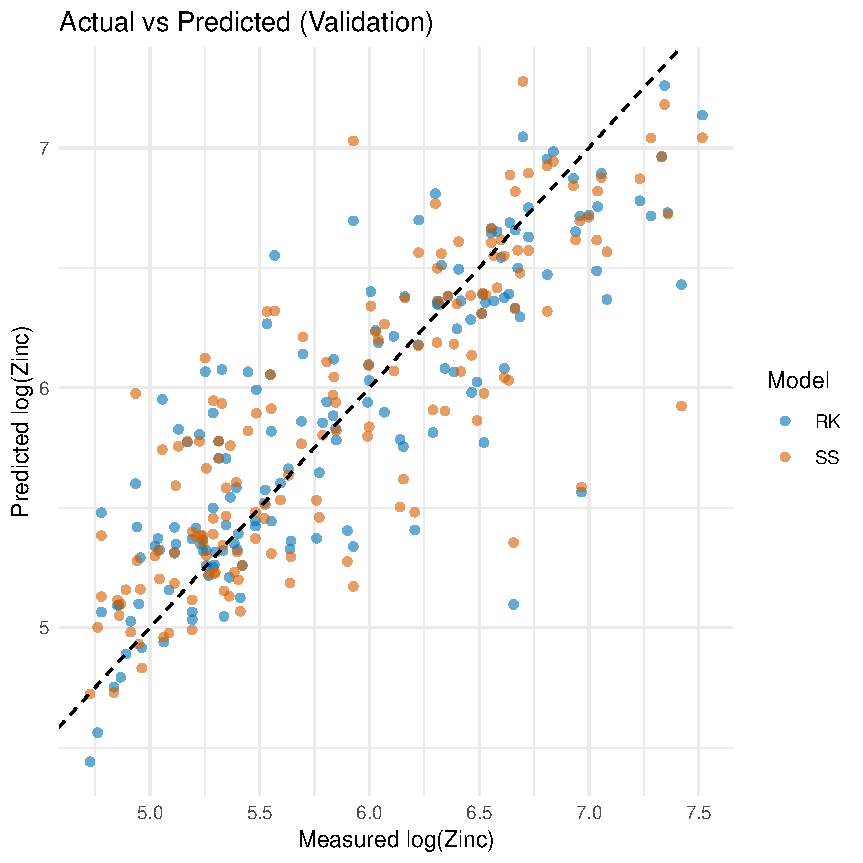
\includegraphics[width=10cm,height=8cm]{Images/fig2.pdf}
\caption{Scatter plot of observed values versus predicted values obtained from the RK and SS models during the validation stage. The dashed line represents the 1:1 line, indicating perfect agreement between observed and predicted values.}
\label{fig2}
\end{figure}
%%%%%%%%%%%%%%%%%%%%%%%% Discussion and Conclusion %%%%%%%%%%%%%%%%%%%%%%%%%%%%%
\section*{Conclusion}
This study compared RK and SS for modeling and mapping zinc (Zn) contamination in the Meuse River basin. The results show that RK provides a more effective framework for representing heavy-metal distributions because it combines the deterministic signal explained by environmental covariates with the spatial dependence remaining in the residuals. SS captured the broad regional pattern well, but its stronger smoothing tended to mute important local variability. In contrast, RK preserved both the overall trend and fine-scale spatial heterogeneity, which was reflected in lower cross-validation errors and clearer, more realistic zonation boundaries.

From a management perspective, these outcomes matter because remediation planning often depends on reliably pinpointing contamination hotspots. In such settings, geostatistical methods such as RK offer a more informative and dependable alternative to approaches based solely on smoothing. More broadly, the findings support the value of hybrid models in environmental geochemistry and provide a solid basis for similar assessments. Future work could further improve performance by incorporating multi-temporal observations and higher-resolution auxiliary data to better capture the long-term dynamics of metal accumulation across river-basin systems.
%\section*{Acknowledgments}
%The authors thank the providers of the Meuse River dataset.

%%%%%%%%%%%%%%%%%%%%%%%% References %%%%%%%%%%%%%%%%%%%%%%%%%%%%%
\begin{thebibliography}{9}

\bibitem[Hengl et al. (2007)]{Hengl2007}
Hengl, T., Heuvelink, G. B., \& Rossiter, D. G. (2007). About regression-kriging: From equations to case studies. {\it Computers \& Geosciences}, 33(10), 1301-1315.

\bibitem[Wahba (1990)]{Wahba1990}
Wahba, G. (1990). {\it Spline models for observational data}. Society for industrial and applied mathematics.

\bibitem[Wood (2017)]{Wood2017}
Wood, S. N. (2017). {\it Generalized Additive Models: An Introduction with R}. CRC press.

\bibitem[R Core Team (2023)]{RCore2023}
R Core Team (2023). {\it R: A language and environment for statistical computing}. R Foundation for Statistical Computing, Vienna, Austria. URL: https://www.R-project.org/.
\end{thebibliography}
\end{document}
